\documentclass[aspectratio=169,11pt]{beamer}

\usepackage[utf8]{inputenc}
\usepackage[T1]{fontenc}
\usepackage[spanish,es-tabla]{babel}
\usepackage{lmodern}
\usepackage{helvet}
\renewcommand{\familydefault}{\sfdefault}

\usepackage{amsmath,amssymb}
\usepackage{booktabs}
\usepackage{colortbl}
\usepackage{array}
\usepackage{graphicx}
\usepackage{xcolor}
\usepackage{tikz}
\usetikzlibrary{arrows.meta,positioning,shapes.geometric,fit,backgrounds,calc}
\usepackage{listings}
\usepackage{hyperref}

% Paleta institucional limpia y de alto contraste
\definecolor{Navy}{HTML}{102A43}
\definecolor{Teal}{HTML}{0F766E}
\definecolor{TealLight}{HTML}{E6F4F1}
\definecolor{BlueSoft}{HTML}{EFF6FF}
\definecolor{Amber}{HTML}{B45309}
\definecolor{AmberLight}{HTML}{FEF3C7}
\definecolor{Coral}{HTML}{B91C1C}
\definecolor{CoralLight}{HTML}{FEE2E2}
\definecolor{Slate}{HTML}{334155}
\definecolor{Muted}{HTML}{64748B}
\definecolor{SoftBg}{HTML}{F8FAFC}
\definecolor{BorderCol}{HTML}{CBD5E1}
\definecolor{RowAlt}{HTML}{F1F5F9}

\usetheme{default}
\usecolortheme{default}
% Mantiene texto en sans-serif (Helvetica) y tipografía matemática serif (Latin Modern Math) para Δ, Γ, Ω sin cuadros negros
\usefonttheme[onlymath]{serif}
\setbeamertemplate{navigation symbols}{}
\setbeamersize{text margin left=0.55cm,text margin right=0.55cm}

\setbeamercolor{normal text}{fg=Navy,bg=white}
\setbeamercolor{frametitle}{fg=white,bg=Navy}
\setbeamercolor{title}{fg=white,bg=Navy}
\setbeamercolor{structure}{fg=Teal}
\setbeamercolor{itemize item}{fg=Teal}
\setbeamercolor{itemize subitem}{fg=Amber}
\setbeamerfont{frametitle}{size=\large,series=\bfseries}
\setbeamerfont{framesubtitle}{size=\footnotesize,series=\normalfont}
\setbeamerfont{title}{size=\Huge,series=\bfseries}
\setbeamerfont{subtitle}{size=\large,series=\normalfont}

\hypersetup{
    colorlinks=true,
    urlcolor=Teal,
    linkcolor=Navy,
    pdftitle={PINN\_V4: Framework Modular POO y Resultados de Campaña},
    pdfauthor={Tesis MIA 2026-2}
}

% Enlaces relativos: oscuro sobre fondo claro (\codelink) y claro sobre fondo Navy (\hdrlink)
\newcommand{\codelink}[2]{\href{run:#1}{\textcolor{Teal}{\underline{\texttt{#2}}}}}
\newcommand{\hdrlink}[2]{\href{run:#1}{\textcolor{AmberLight}{\underline{\texttt{#2}}}}}
\newcommand{\badge}[1]{\tikz[baseline=(X.base)]{\node[fill=TealLight,draw=Teal!60,rounded corners=2pt,inner xsep=4pt,inner ysep=1.2pt,font=\scriptsize\bfseries,text=Teal] (X) {#1};}}

% Caja visual ligera y compacta compatible con MiKTeX base
\newenvironment{cardbox}[2][Teal]{%
  \begin{tikzpicture}
    \node[draw=#1!65,fill=SoftBg,rounded corners=4pt,line width=0.8pt,inner sep=4.5pt,text width=\dimexpr\linewidth-11pt\relax,align=left] \bgroup
    {\color{#1}\bfseries #2}\par\vspace{1pt}%
}{%
    \egroup;
  \end{tikzpicture}%
}

% Listas compactas dentro de tarjetas para aprovechar el formato 16:9
\newenvironment{citemize}{%
  \begin{itemize}\setlength\itemsep{2pt}\setlength\parskip{0pt}\setlength\parsep{0pt}\vspace{-2pt}%
}{%
  \end{itemize}\vspace{-2pt}%
}

% Estilo listings para JSON con soporte UTF-8 español
\lstset{
  basicstyle=\ttfamily\fontsize{6.8}{7.8}\selectfont,
  backgroundcolor=\color{SoftBg},
  frame=single,
  rulecolor=\color{BorderCol},
  breaklines=true,
  columns=fullflexible,
  showstringspaces=false,
  literate={á}{{\'a}}1 {é}{{\'e}}1 {í}{{\'i}}1 {ó}{{\'o}}1 {ú}{{\'u}}1
           {Á}{{\'A}}1 {É}{{\'E}}1 {Í}{{\'I}}1 {Ó}{{\'O}}1 {Ú}{{\'U}}1
           {ñ}{{\~n}}1 {Ñ}{{\~N}}1
}

% Encabezado y pie compactos
\setbeamertemplate{frametitle}{%
  \nointerlineskip%
  \begin{beamercolorbox}[wd=\paperwidth,ht=0.88cm,dp=0.14cm,leftskip=0.55cm,rightskip=0.55cm]{frametitle}%
    \usebeamerfont{frametitle}\insertframetitle\par
    \ifx\insertframesubtitle\@empty\else
      {\usebeamerfont{framesubtitle}\color{TealLight}\insertframesubtitle}%
    \fi
  \end{beamercolorbox}%
}

\setbeamertemplate{footline}{%
  \begin{beamercolorbox}[wd=\paperwidth,ht=0.40cm,dp=0.10cm,leftskip=0.55cm,rightskip=0.55cm]{normal text}%
    \color{BorderCol}\rule{\dimexpr\paperwidth-1.1cm\relax}{0.4pt}\par\vspace{1.5pt}
    {\scriptsize\color{Muted}\textbf{PINN\_V4} (\codelink{../README.md}{pinn-thermal}) \textbar\ \insertsectionhead \hfill Diapositiva \insertframenumber\ / \inserttotalframenumber}
  \end{beamercolorbox}%
}

% Portadilla de sección sin cortes de palabra incómodos
\newcommand{\sectionbanner}[3]{%
  \begin{frame}[plain]
    \begin{tikzpicture}[remember picture,overlay]
      \fill[Navy] (current page.south west) rectangle (current page.north east);
      \fill[Teal] (current page.south west) rectangle ($(current page.north west)+(0.45cm,0)$);
      \node[anchor=north west,text=TealLight,font=\large\bfseries,align=left,text width=13.2cm] (K) at ($(current page.north west)+(1.3cm,-2.0cm)$) {#1};
      \node[anchor=north west,text=white,font=\fontsize{26}{30}\selectfont\bfseries,align=left,text width=13.2cm] (T) at ($(K.south west)+(0,-0.35cm)$) {\raggedright #2};
      \node[anchor=north west,text=BorderCol,font=\large,align=left,text width=13.2cm] at ($(T.south west)+(0,-0.45cm)$) {\raggedright #3};
    \end{tikzpicture}
  \end{frame}
}

\begin{document}

% ==============================================================================
% SLIDE 1: PORTADA
% ==============================================================================
\begin{frame}[plain]
  \begin{tikzpicture}[remember picture,overlay]
    \fill[Navy] (current page.south west) rectangle (current page.north east);
    \fill[Teal] (current page.south west) rectangle ($(current page.north west)+(0.5cm,0)$);
    \node[anchor=north west,text=TealLight,font=\normalsize\bfseries,text width=13.6cm,align=left] (K1) at ($(current page.north west)+(1.25cm,-0.80cm)$)
      {TESIS MIA 2026-2 \textbar\ ARQUITECTURA DE SOFTWARE Y RESULTADOS};
    \node[anchor=north west,text=white,font=\fontsize{22}{26}\selectfont\bfseries,text width=13.6cm,align=left] (T1) at ($(K1.south west)+(0,-0.25cm)$)
      {\raggedright PINN\_V4 (\texttt{pinn\_thermal}): Framework POO para Problemas Térmicos 2D en Cables Subterráneos};
    \node[anchor=north west,text=BorderCol,font=\large,text width=13.6cm,align=left] (S1) at ($(T1.south west)+(0,-0.30cm)$)
      {\raggedright Núcleo desacoplado de física JSON, motores PINN y FEM P2 (FEniCSx/WSL2), campaña en embudo, catálogo de modelos y front-end Streamlit.};
    \node[anchor=north west,fill=SoftBg,rounded corners=4pt,inner sep=7pt,font=\footnotesize,text width=13.4cm,align=left] (B1) at ($(S1.south west)+(0,-0.45cm)$)
      {\textbf{Accesos:} \codelink{../README.md}{README.md} \textbar\ \codelink{../docs/arquitectura.md}{arquitectura.md} \textbar\ \codelink{../docs/detalle_tecnico_implementaciones_pinn.md}{detalle\_tecnico\_pinn.md}\\[2pt]
      \codelink{../frontend/app.py}{frontend/app.py} \textbar\ \href{run:launch_frontend.bat}{\textcolor{Amber}{\underline{\textbf{Arrancar Front-End}}}} \textbar\ \href{http://localhost:8501}{\textcolor{Teal}{\underline{\texttt{http://localhost:8501}}}}};
  \end{tikzpicture}
\end{frame}

% ==============================================================================
% SLIDE 2: AGENDA EN 3 PARTES
% ==============================================================================
\section{Visión General}
\begin{frame}{Estructura de la Presentación}
  \framesubtitle{Tres bloques para explicar ingeniería del software, fundamentos PINN y avance experimental}
  \small
  \begin{columns}[T,totalwidth=\textwidth]
    \begin{column}{0.32\textwidth}
      \begin{cardbox}[Teal]{Parte I: Ingeniería y Flujo}
        \begin{citemize}
          \item Estructura del proyecto POO
          \item Capas de \texttt{pinn\_thermal}
          \item Flujo de llamado a funciones
          \item Esquema JSON única verdad
          \item Motor PINN y Motor FEM P2
          \item Campaña en embudo (\texttt{00}--\texttt{05})
          \item Front-End Streamlit + lanzador
        \end{citemize}
      \end{cardbox}
    \end{column}
    \begin{column}{0.32\textwidth}
      \begin{cardbox}[Navy]{Parte II: Modelos PINN}
        \begin{citemize}
          \item Línea base \texttt{M0} y \texttt{M0R}
          \item Subdominios \texttt{M1} (cPINN/XPINN)
          \item Mixta 1er orden \texttt{M2} (FO-PINN)
          \item Cúspides \texttt{CUSP} / \texttt{CUSPR}
          \item Discontinuos \texttt{DCSNN}
          \item Bases finitas \texttt{FBPINN} ($C^2$)
          \item Exactos \texttt{M1\_EXACT} / \texttt{CUSP\_EXACT}
          \item DeepXDE + tabla resumen
        \end{citemize}
      \end{cardbox}
    \end{column}
    \begin{column}{0.32\textwidth}
      \begin{cardbox}[Amber]{Parte III: Campaña Actual}
        \begin{citemize}
          \item Etapa 0: 9 MMS + 29 FEM P2
          \item Etapa 1: Smoke 10 modelos (40/40)
          \item Etapa 2: \texttt{CON} vs \texttt{SIN energy}
          \item Ranking curado y poda
          \item Promovidos: \texttt{M0R, M1, FBPINN, M2, DCSNN}
          \item Etapa 3 en curso y hoja de ruta (\texttt{04} y \texttt{05})
        \end{citemize}
      \end{cardbox}
    \end{column}
  \end{columns}
\end{frame}

% ==============================================================================
% PARTE I: SOFTWARE, MOTORES, JSON, CAMPAÑAS Y FRONT-END
% ==============================================================================
\sectionbanner{PARTE I}{Ingeniería del Software, Motores y Campañas}{Diseño modular POO, flujo de ejecución, formato JSON, FEniCSx WSL2 y Front-End}

\section{Parte I: Software y Motores}

% SLIDE 3: ESTRUCTURA DEL PROYECTO
\begin{frame}{Estructura del Proyecto y Principios POO}
  \framesubtitle{Separación estricta entre dominio físico JSON, resolvedores, evaluación FEM, notebooks y UI}
  \begin{columns}[T,totalwidth=\textwidth]
    \begin{column}{0.53\textwidth}
      \resizebox{\linewidth}{!}{%
      \begin{tikzpicture}[
        node distance=0.20cm and 0.35cm,
        box/.style={draw=Navy!70,fill=SoftBg,rounded corners=3pt,minimum width=3.2cm,minimum height=0.52cm,font=\small\bfseries,align=center},
        sub/.style={draw=Teal!60,fill=TealLight!50,rounded corners=3pt,text width=6.1cm,minimum height=0.48cm,font=\footnotesize,align=left}
      ]
        \node[box,fill=Navy,text=white] (root) {\texttt{tesis\_MIA\_2026-2\_pinn/}};
        \node[sub,below right=0.18cm and -1.8cm of root] (src) {\textbf{\texttt{src/pinn\_thermal/}}: librería principal POO};
        \node[sub,below=0.12cm of src] (cases) {\textbf{\texttt{cases/}}: 12 benchmarks + 17 casos curados JSON};
        \node[sub,below=0.12cm of cases] (nb) {\textbf{\texttt{notebooks\_campaign/}}: embudo Etapas 0--5};
        \node[sub,below=0.12cm of nb] (fe) {\textbf{\texttt{frontend/}}: app multipágina Streamlit};
        \node[sub,below=0.12cm of fe] (docs) {\textbf{\texttt{docs/}} y \textbf{\texttt{tests/}}: manuales + 43 tests};
        \draw[-{Stealth[length=2mm]},Navy!70,thick] (root.south) |- (src.west);
        \draw[-{Stealth[length=2mm]},Navy!70,thick] (root.south) |- (cases.west);
        \draw[-{Stealth[length=2mm]},Navy!70,thick] (root.south) |- (nb.west);
        \draw[-{Stealth[length=2mm]},Navy!70,thick] (root.south) |- (fe.west);
        \draw[-{Stealth[length=2mm]},Navy!70,thick] (root.south) |- (docs.west);
      \end{tikzpicture}}
    \end{column}
    \begin{column}{0.45\textwidth}
      \begin{cardbox}[Teal]{Contratos clave de diseño}
        \small
        \begin{citemize}
          \item \textbf{Sin lógica \textit{ad hoc}}: cada solver recibe solo un \texttt{ThermalProblem2D} desde JSON.
          \item \textbf{Polimorfismo uniforme}: toda arquitectura hereda de \texttt{BasePINNModel} vía \texttt{ModelRegistry}.
          \item \textbf{Agnóstico a hardware}: CPU, CUDA, Intel XPU, NPU y MPS (\texttt{DeviceManager}).
        \end{citemize}
      \end{cardbox}
      \vspace{0.10cm}
      {\small Links: \codelink{../src/pinn_thermal/}{src/pinn\_thermal/} \textbar\ \codelink{../cases/}{cases/} \textbar\ \codelink{../tests/}{tests/}}
    \end{column}
  \end{columns}
\end{frame}

% SLIDE 4: ARQUITECTURA POR CAPAS
\begin{frame}{Arquitectura Modular por Capas de \texttt{pinn\_thermal}}
  \framesubtitle{Capas desacopladas: el dominio y el trabajador FEM no dependen de PyTorch}
  \centering
  \resizebox{0.84\textwidth}{!}{%
  \begin{tikzpicture}[
    layer/.style={draw=Navy!75,rounded corners=4pt,text width=12.6cm,minimum height=0.58cm,align=center,font=\small},
    hlayer/.style={draw=Navy!75,rounded corners=4pt,text width=5.95cm,minimum height=0.60cm,align=center,font=\small},
    arr/.style={-{Stealth[length=2.2mm]},thick,Navy!80}
  ]
    \node[layer,fill=Navy,text=white] (L4) {\textbf{Capa 4 — Interfaces:} Streamlit (\hdrlink{../frontend/app.py}{frontend/}), CLI (\texttt{pinn-thermal}) y Cuadernos (\hdrlink{../notebooks_campaign/}{notebooks\_campaign/})};
    \node[layer,fill=BlueSoft,below=0.14cm of L4] (L3) {\textbf{Capa 3 — Visualización y Edición:} mallas, cortes, Plotly/Matplotlib, \texttt{CaseEditorHelper}};
    \node[hlayer,fill=TealLight,below=0.14cm of L3,xshift=-3.32cm] (L2) {\textbf{Capa 2 — Modelos PINN:} \codelink{../src/pinn_thermal/models/baseline.py}{models/} (\texttt{BasePINNModel})};
    \node[hlayer,fill=AmberLight,below=0.14cm of L3,xshift=3.32cm] (FEM) {\textbf{Motor FEM Externo:} \codelink{../src/pinn_thermal/fem/runner.py}{fem/} (Gmsh+DolfinX, sin PyTorch)};
    \coordinate (mid2) at ($(L2.south)!0.5!(FEM.south)$);
    \node[layer,fill=SoftBg,below=0.20cm of mid2] (L1B) {\textbf{Capa 1B — Motor PyTorch:} \texttt{DeviceManager}, \texttt{ParallelRunner}, \texttt{PhysicsObjective}, \texttt{PINNTrainer}, \texttt{SolutionArtifact}};
    \node[layer,fill=RowAlt,below=0.14cm of L1B] (L1A) {\textbf{Capa 1A — Dominio Puro (sin PyTorch):} AST \texttt{expressions}, \texttt{fields}, \texttt{shapes}, \texttt{schema}, \texttt{ThermalProblem2D}};

    \draw[arr] (L4) -- (L3);
    \draw[arr] (L3.south -| L2) -- (L2.north);
    \draw[arr] (L3.south -| FEM) -- (FEM.north);
    \draw[arr] (L2.south) -- (L1B.north -| L2);
    \draw[arr] (FEM.east) -- ++(0.32cm,0) |- (L1A.east);
    \draw[arr] (L1B) -- (L1A);
  \end{tikzpicture}}
  \vspace{0.08cm}
  {\footnotesize Ver \codelink{../docs/arquitectura.md}{docs/arquitectura.md} \textbar\ La Capa 1A puede validarse, editarse y traducirse a UFL sin inicializar \texttt{torch}.}
\end{frame}

% SLIDE 5: FLUJO DE LLAMADO A FUNCIONES Y CLASES
\begin{frame}{Estructura de Llamado a Funciones y Clases (\textit{End-to-End})}
  \framesubtitle{Desde el archivo JSON del problema hasta el artefacto portable y su evaluación auditada}
  \centering
  \resizebox{0.96\textwidth}{!}{%
  \begin{tikzpicture}[
    node distance=0.38cm and 0.28cm,
    fstep/.style={draw=Teal!80,fill=SoftBg,rounded corners=4pt,text width=3.45cm,minimum height=1.10cm,align=center,font=\footnotesize,line width=0.8pt},
    arr/.style={-{Stealth[length=2.2mm]},thick,Navy}
  ]
    \node[fstep] (S1) {\textbf{1. Carga JSON}\\\texttt{CaseCatalog.load()}\\\texttt{ThermalProblem2D}\\(\codelink{../src/pinn_thermal/core/problem.py}{problem.py})};
    \node[fstep,right=of S1] (S2) {\textbf{2. Modelo OOP}\\\texttt{ModelRegistry.build()}\\\texttt{model.field(r, xy)}\\(\codelink{../src/pinn_thermal/core/base_model.py}{base\_model.py})};
    \node[fstep,right=of S2] (S3) {\textbf{3. Física}\\\texttt{PhysicsObjective()}\\\texttt{collocation + loss}\\(\codelink{../src/pinn_thermal/core/objective.py}{objective.py})};
    \node[fstep,right=of S3] (S4) {\textbf{4. Entrenador}\\\texttt{PINNTrainer.train()}\\\texttt{Adam -> L-BFGS}\\(\codelink{../src/pinn_thermal/core/trainer.py}{trainer.py})};

    \node[fstep,below=0.36cm of S4] (S5) {\textbf{5. Persistencia}\\\texttt{SolutionArtifact}\\\texttt{model.pt + result.json}\\(\codelink{../src/pinn_thermal/core/artifact.py}{artifact.py})};
    \node[fstep,left=of S5] (S6) {\textbf{6. Auditoría}\\\texttt{evaluate\_model()}\\\texttt{NRMSE, dTmax, bal}\\(\codelink{../src/pinn_thermal/core/evaluation.py}{evaluation.py})};
    \node[fstep,left=of S6] (S7) {\textbf{7. Continuación}\\\texttt{Weight / Functional}\\\texttt{ChainedPINN}\\(\codelink{../src/pinn_thermal/core/transfer.py}{transfer.py})};
    \node[fstep,left=of S7] (S8) {\textbf{8. Ingeniería}\\\texttt{ampacity.py}\\Bisección $I_{\max}$\\(\codelink{../src/pinn_thermal/core/ampacity.py}{ampacity.py})};

    \draw[arr] (S1) -- (S2);
    \draw[arr] (S2) -- (S3);
    \draw[arr] (S3) -- (S4);
    \draw[arr] (S4) -- (S5);
    \draw[arr] (S5) -- (S6);
    \draw[arr] (S6) -- (S7);
    \draw[arr] (S7) -- (S8);
  \end{tikzpicture}}
  \vspace{0.10cm}
  \begin{cardbox}[Navy]{Ejecución multi-tarea transparente}
    \small \texttt{ParallelRunner} (\codelink{../src/pinn_thermal/core/parallel.py}{parallel.py}) encapsula listas de \texttt{RunTask} o \texttt{AdaptiveRunTask} con contexto \texttt{spawn}, balanceo de hilos CPU/GPUs y tablero HTML en vivo leyendo \texttt{progress.json}.
  \end{cardbox}
\end{frame}

% SLIDE 6: FORMATO DE INGRESO JSON
\begin{frame}[fragile]{Formato de Ingreso de Datos JSON (\texttt{pinn-v4-problem-1})}
  \framesubtitle{Única fuente de verdad geométrica y física compartida por todos los solvers PINN y FEM}
  \begin{columns}[T,totalwidth=\textwidth]
    \begin{column}{0.49\textwidth}
\begin{lstlisting}[basicstyle=\ttfamily\fontsize{6.8}{7.8}\selectfont]
{
  "schema": "pinn-v4-problem-1",
  "id": "xlpe_discrete_layers",
  "family": "cable", "temperature_scale_K": 50.0,
  "domain": {"shape": "rectangle", "bounds": [-4, 4, -3, 0]},
  "boundaries": {
    "top": {"type": "robin", "h_W_m2K": 10.0, "T_inf_C": 20.0},
    "bottom": {"type": "dirichlet", "value": 20.0},
    "left": {"type": "neumann", "q_n_W_m2": 0.0},
    "right": {"type": "neumann", "q_n_W_m2": 0.0}
  },
  "regions": [
    {"id": "soil", "priority": 0, "shape": {...}, "conductivity": 1.0},
    {"id": "cond", "priority": 5, "shape": {"type": "disk", ...}, "source": 5e5}
  ]
}
\end{lstlisting}
    \end{column}
    \begin{column}{0.48\textwidth}
      \begin{cardbox}[Teal]{Capacidades del esquema}
        \footnotesize
        \begin{citemize}
          \item \textbf{4 geometrías}: \texttt{rectangle}, \texttt{disk}, \texttt{annulus}, \texttt{polygon} con \texttt{area()} exacta (\codelink{../src/pinn_thermal/core/shapes.py}{shapes.py}).
          \item \textbf{Regla \texttt{priority}}: mayor entero manda en solapes (cables concéntricos).
          \item \textbf{7 campos} (\codelink{../src/pinn_thermal/core/fields.py}{fields.py}): constante, \texttt{expr(x,y)}, \texttt{piecewise}, \texttt{table} 1D/2D, \texttt{layers}, \texttt{patch}.
          \item \textbf{BCs generales}: Dirichlet, Neumann saliente y Robin en cualquier borde.
        \end{citemize}
      \end{cardbox}
      \vspace{0.08cm}
      {\footnotesize Manual: \codelink{../docs/formato_json.md}{formato\_json.md} \textbar\ Casos: \codelink{../cases/thesis_curated/xlpe_discrete_layers/problem.json}{xlpe\_discrete}, \codelink{../cases/thesis_curated/aras_flat/problem.json}{aras\_flat}}
    \end{column}
  \end{columns}
\end{frame}

% SLIDE 7: MOTOR PINN (OBJECTIVE + TRAINER + PARALELISMO)
\begin{frame}{Motor PINN: Objetivo Adimensional y Entrenamiento Híbrido}
  \framesubtitle{Normalización automática de Fourier por subregión, parada por divergencia y soporte multi-dispositivo}
  \centering
  \resizebox{0.97\textwidth}{!}{%
  \begin{tikzpicture}[
    blk/.style={draw=Navy!75,fill=SoftBg,rounded corners=4pt,minimum height=0.92cm,align=center,font=\footnotesize,line width=0.8pt},
    arr/.style={-{Stealth[length=2mm]},thick,Teal}
  ]
    \node[blk,fill=TealLight,text width=3.2cm] (P1) {\textbf{Colocación Mixta}\\Interior, capa, interfaz,\\frontera (resample focalizado)};
    \node[blk,right=0.38cm of P1,text width=3.9cm] (P2) {\textbf{Residuos Adimensionales}\\\texttt{pde}, \texttt{constitutive}, \texttt{dirichlet},\\\texttt{neumann}, \texttt{robin}, \texttt{interface\_flux}, \texttt{energy}};
    \node[blk,right=0.38cm of P2,fill=BlueSoft,text width=2.9cm] (P3) {\textbf{Fase 1: Adam}\\+ \texttt{CosineAnnealingLR}\\+ \texttt{DivergenceGuard}};
    \node[blk,right=0.38cm of P3,fill=AmberLight,text width=2.7cm] (P4) {\textbf{Fase 2: L-BFGS}\\\texttt{strong\_wolfe}\\+ \texttt{AccuracyStop}};
    \draw[arr] (P1) -- (P2);
    \draw[arr] (P2) -- (P3);
    \draw[arr] (P3) -- (P4);
  \end{tikzpicture}}
  \vspace{0.14cm}
  \begin{columns}[T,totalwidth=\textwidth]
    \begin{column}{0.49\textwidth}
      \begin{cardbox}[Teal]{Correcciones (\codelink{../src/pinn_thermal/core/objective.py}{objective.py})}
        \small
        \begin{citemize}
          \item \textbf{\texttt{interface\_flux = 100.0} obligatorio}: evita desacoplamiento cable-suelo incluso si $[T]=0$ exacto.
          \item \textbf{Capas delgadas}: respaldo local de 4096 pts para $\Delta T_{\text{local},r}$ y área exacta en anillos de $1\text{ mm}$.
        \end{citemize}
      \end{cardbox}
    \end{column}
    \begin{column}{0.49\textwidth}
      \begin{cardbox}[Navy]{Hardware y paralelismo (\codelink{../src/pinn_thermal/core/device.py}{device.py})}
        \small
        \begin{citemize}
          \item \textbf{Backends}: CPU, CUDA, Intel XPU (parche nativo \texttt{aten::dot} para L-BFGS), ROCm, NPU, MPS.
          \item \textbf{Atención opcional}: RBA / Self-Adaptive (\texttt{attention.py}) cuando \texttt{lbfgs\_steps=0}.
        \end{citemize}
      \end{cardbox}
    \end{column}
  \end{columns}
\end{frame}

% SLIDE 8: ARTEFACTO PORTABLE Y RUTAS DE CONTINUACIÓN
\begin{frame}{Artefacto Único \texttt{SolutionArtifact} y Transferencia}
  \framesubtitle{Interoperabilidad total entre CLI, Jupyter y Streamlit + cuatro estrategias de continuación}
  \begin{columns}[T,totalwidth=\textwidth]
    \begin{column}{0.47\textwidth}
      \begin{cardbox}[Navy]{Formato \texttt{pinn-v4-artifact-1} (\codelink{../src/pinn_thermal/core/artifact.py}{artifact.py})}
        \small Cada corrida persiste atómicamente:
        \begin{citemize}
          \item \texttt{problem.json} + \texttt{specification.json} (SHA-256)
          \item \texttt{model.pt}: pesos + estado completo Adam/RNG/nubes
          \item \texttt{result.json}: métricas, historia y auditoría física
          \item \texttt{manifest.json} + exportación portable \texttt{.zip}
        \end{citemize}
      \end{cardbox}
    \end{column}
    \begin{column}{0.51\textwidth}
      \resizebox{\linewidth}{!}{%
      \begin{tikzpicture}[
        node distance=0.18cm,
        rt/.style={draw=Teal!70,fill=TealLight!45,rounded corners=3pt,text width=6.6cm,inner sep=4.5pt,font=\footnotesize,align=left}
      ]
        \node[rt] (R1) {\textbf{1. \texttt{resume\_from}}: reanudación bit-exacta de bloques \texttt{adam -> lbfgs} (Etapa 4A).};
        \node[rt,below=of R1] (R2) {\textbf{2. \texttt{warm\_start\_from}}: \texttt{WeightTransfer} compatible o \texttt{FunctionalTransfer} (\texttt{readout} / \texttt{pretrain}).};
        \node[rt,below=of R2] (R3) {\textbf{3. \texttt{chain\_from}}: \texttt{ChainedPINN} aditivo (\texttt{residual}) o enriquecimiento (\texttt{feature}).};
        \node[rt,below=of R3] (R4) {\textbf{4. \texttt{initializer}}: arranque discreto \texttt{RBFFDInitializer} o \texttt{FEMInitializer}.};
      \end{tikzpicture}}
      \vspace{0.08cm}
      {\footnotesize Ver \codelink{../src/pinn_thermal/core/transfer.py}{transfer.py} y \codelink{../src/pinn_thermal/models/rbf_init.py}{rbf\_init.py}.}
    \end{column}
  \end{columns}
\end{frame}

% SLIDE 9: MOTOR FEM P2 E INTERPOLACIÓN VECTORIZADA
\begin{frame}{Motor FEM de Referencia (\texttt{FEniCSxAdapter}) e Interpolación P2}
  \framesubtitle{Generación externa en WSL2 sin PyTorch e interpolación P2 vectorizada 800$\times$--2,300$\times$ más rápida}
  \centering
  \resizebox{0.97\textwidth}{!}{%
  \begin{tikzpicture}[
    blk/.style={draw=Amber!80!black,fill=AmberLight!55,rounded corners=4pt,minimum height=0.92cm,align=center,font=\footnotesize,line width=0.8pt},
    arr/.style={-{Stealth[length=2mm]},thick,Navy}
  ]
    \node[blk,text width=2.8cm] (F1) {\textbf{1. Traducción UFL}\\\texttt{ufl\_backend.py}\\(\codelink{../src/pinn_thermal/fem/ufl_backend.py}{ufl\_backend.py})};
    \node[blk,right=0.38cm of F1,text width=3.2cm] (F2) {\textbf{2. Mallado Gmsh P2}\\Transiciones y refinamiento\\(\codelink{../src/pinn_thermal/fem/mesh_resolution.py}{mesh\_resolution.py})};
    \node[blk,right=0.38cm of F2,text width=3.1cm] (F3) {\textbf{3. Worker WSL2}\\DolfinX lineal/Picard\\(\codelink{../src/pinn_thermal/fem/worker.py}{worker.py})};
    \node[blk,right=0.38cm of F3,fill=TealLight,draw=Teal,text width=3.2cm] (F4) {\textbf{4. Caché + MLS P2}\\\texttt{fem\_l1.json/.npz}\\+ \texttt{eval\_ref\_T.npz}};
    \draw[arr] (F1) -- (F2);
    \draw[arr] (F2) -- (F3);
    \draw[arr] (F3) -- (F4);
  \end{tikzpicture}}
  \vspace{0.14cm}
  \begin{columns}[T,totalwidth=\textwidth]
    \begin{column}{0.52\textwidth}
      \begin{cardbox}[Teal]{Aceleración (\codelink{../src/pinn_thermal/core/artifact.py}{artifact.py})}
        \small
        \begin{citemize}
          \item \texttt{LinearNDInterpolator} caía en $O(N^2)$ sobre mallas multi-región con huecos (19 min en \texttt{kim\_2024} y horas en 3.8M DOFs).
          \item Reemplazado por \textbf{MLS P2 vectorizado sobre \texttt{cKDTree}} (\texttt{workers=-1}) por región.
        \end{citemize}
      \end{cardbox}
    \end{column}
    \begin{column}{0.46\textwidth}
      \begin{cardbox}[Navy]{Tiempos reales medidos (\texttt{art.predict})}
        \footnotesize
        \begin{tabular}{@{}lrr@{}}
          \toprule
          Caso & Antes & Ahora \\
          \midrule
          \texttt{cable\_disk} & 18.6 s & \textbf{0.023 s} \\
          \texttt{xlpe\_discrete\_layers} & 170 s & \textbf{0.073 s} \\
          \texttt{aras\_flat} & 499 s & \textbf{0.221 s} \\
          \texttt{kim\_2024\_original} & 1,140 s & \textbf{1.176 s} \\
          \bottomrule
        \end{tabular}
      \end{cardbox}
    \end{column}
  \end{columns}
\end{frame}

% SLIDE 10: ESTRUCTURA DE CAMPAÑAS EN EMBUDO
\begin{frame}{Estructura de Campañas Reproducibles en Embudo}
  \framesubtitle{Seis cuadernos Jupyter secuenciales (\hdrlink{../notebooks_campaign/}{notebooks\_campaign/}) con \texttt{OVERWRITE = False} y caché atómica}
  \centering
  \resizebox{0.97\textwidth}{!}{%
  \begin{tikzpicture}[
    st/.style={draw=Navy!75,fill=SoftBg,rounded corners=3pt,text width=2.05cm,minimum height=1.20cm,align=center,font=\scriptsize,line width=0.8pt},
    arr/.style={-{Stealth[length=1.8mm]},thick,Teal}
  ]
    \node[st,fill=RowAlt] (N0) {\textbf{Etapa 0}\\Auditoría MMS\\+ FEM P2 WSL2\\\codelink{../notebooks_campaign/00_auditoria_y_referencias_fem_wsl.ipynb}{00\_auditoria}};
    \node[st,right=0.22cm of N0] (N1) {\textbf{Etapa 1}\\Smoke 10 archs\\4 casos pivote\\\codelink{../notebooks_campaign/01_smoke_test_arquitecturas.ipynb}{01\_smoke}};
    \node[st,right=0.22cm of N1,fill=TealLight] (N2) {\textbf{Etapa 2}\\Screening dual\\CON/SIN energy\\\codelink{../notebooks_campaign/02_screening_seleccion_modelos_1200_50.ipynb}{02\_screening}};
    \node[st,right=0.22cm of N2] (N3) {\textbf{Etapa 3}\\29 casos $\times$ 3 seeds\\Top 5 promovidos\\\codelink{../notebooks_campaign/03_smoke_multicaso_semillas.ipynb}{03\_multicaso}};
    \node[st,right=0.22cm of N3] (N4) {\textbf{Etapa 4}\\4A Adaptativo\\4B Largas 8000+20\\\codelink{../notebooks_campaign/04_campana_adaptativa_y_corridas_largas.ipynb}{04\_campana}};
    \node[st,right=0.22cm of N4,fill=AmberLight] (N5) {\textbf{Etapa 5}\\Clasificación\\Reporte + UI\\\codelink{../notebooks_campaign/05_clasificacion_resultados_y_reporte_tesis.ipynb}{05\_reporte}};
    \draw[arr] (N0)--(N1); \draw[arr] (N1)--(N2); \draw[arr] (N2)--(N3); \draw[arr] (N3)--(N4); \draw[arr] (N4)--(N5);
  \end{tikzpicture}}
  \vspace{0.12cm}
  \begin{columns}[T,totalwidth=\textwidth]
    \begin{column}{0.49\textwidth}
      \begin{cardbox}[Teal]{Banderas de control y reanudación}
        \small
        \begin{citemize}
          \item \texttt{RUN\_MODE}: \texttt{''demo\_fast''} vs \texttt{''full\_campaign''}.
          \item \texttt{OVERWRITE = False}: lee \texttt{summary.json}/\texttt{result.json} y solo ejecuta corridas faltantes.
          \item \texttt{USE\_PARALLEL}: CPU paralelo (\texttt{spawn}) vs \texttt{XPU/CUDA}.
        \end{citemize}
      \end{cardbox}
    \end{column}
    \begin{column}{0.49\textwidth}
      \begin{cardbox}[Navy]{Criterios oficiales de calificación}
        \small
        \begin{citemize}
          \item \textbf{STRICT}: $|\Delta T_{\max}| < 0.05\text{ K}$, $\text{NRMSE} < 0.25\%$, $\text{bal} < 0.5\%$.
          \item \textbf{RELAXED} (4A): $2\times \text{STRICT}$ para saltar temprano a \texttt{L-BFGS}.
          \item \textbf{Compuerta Etapa 2}: sanidad \texttt{mms\_sine} + $\max\text{bal} < 50\%$.
        \end{citemize}
      \end{cardbox}
    \end{column}
  \end{columns}
\end{frame}

% SLIDE 11: FRONT-END STREAMLIT + BOTONES DE ARRANQUE Y CONEXIÓN
\begin{frame}{Front-End Web Interactivo en Streamlit}
  \framesubtitle{Lanzamiento: \texttt{streamlit run frontend/app.py} o \texttt{pinn-thermal ui} (\hdrlink{../frontend/README.md}{frontend/README.md})}
  \centering
  \resizebox{0.84\textwidth}{!}{%
  \begin{tikzpicture}[
    view/.style={draw=Teal!80,fill=SoftBg,rounded corners=4pt,text width=6.0cm,minimum height=1.30cm,align=left,inner sep=5pt,font=\footnotesize,line width=0.8pt},
    hub/.style={draw=Navy,fill=Navy,text=white,rounded corners=4pt,minimum width=4.8cm,minimum height=0.62cm,font=\small\bfseries,align=center}
  ]
    \node[hub] (ST) at (0,0) {\texttt{WorkspaceStore} (\hdrlink{../frontend/state.py}{state.py})};
    \node[view] (V1) at (-3.55, 1.50) {\textbf{1. Estudio de Casos (\codelink{../frontend/views/case_studio.py}{case\_studio.py})}\\Creación guiada/JSON, materiales, heterogeneidades (tabla, capas, parches) y visor Plotly.};
    \node[view] (V2) at ( 3.55, 1.50) {\textbf{2. Ejecutor (\codelink{../frontend/views/runner_view.py}{runner\_view.py})}\\Entrena PINN, \texttt{resume}, transferencia, \texttt{ChainedPINN}, FEniCSx WSL2 y ampacidad.};
    \node[view] (V3) at (-3.55,-1.50) {\textbf{3. Comparador (\codelink{../frontend/views/compare_view.py}{compare\_view.py})}\\Contrasta corridas de Streamlit, Jupyter o CLI en \texttt{frontend/workspace/runs/}.};
    \node[view] (V4) at ( 3.55,-1.50) {\textbf{4. Teoría y Auditoría (\codelink{../frontend/views/docs_view.py}{docs\_view.py})}\\Catálogo vivo \texttt{ModelRegistry}, teoría matemática, auditoría frente a papers y JSON.};
    \draw[thick,Teal] (V1.south) -- (ST.north west);
    \draw[thick,Teal] (V2.south) -- (ST.north east);
    \draw[thick,Teal] (V3.north) -- (ST.south west);
    \draw[thick,Teal] (V4.north) -- (ST.south east);
  \end{tikzpicture}}
  \vspace{0.16cm}
  \begin{center}
    \href{run:launch_frontend.bat}{\tikz[baseline=(B1.base)]{\node[fill=Teal,draw=Teal!80!black,rounded corners=4pt,inner xsep=10pt,inner ysep=5pt,font=\small\bfseries,text=white] (B1) {Arrancar Front-End (\texttt{launch\_frontend.bat})};}}
    \hspace{0.45cm}
    \href{http://localhost:8501}{\tikz[baseline=(B2.base)]{\node[fill=Navy,draw=Navy!80!black,rounded corners=4pt,inner xsep=10pt,inner ysep=5pt,font=\small\bfseries,text=white] (B2) {Conectar al Front-End (\texttt{http://localhost:8501})};}}
  \end{center}
\end{frame}

% ==============================================================================
% PARTE II: MODELOS PINN IMPLEMENTADOS
% ==============================================================================
\sectionbanner{PARTE II}{Modelos PINN Implementados}{Fundamentos físicos, papers fundacionales, modificaciones del proyecto, pros y contras}

\section{Parte II: Modelos PINN}

% SLIDE 12: MAPA DE MODELOS REGISTRADOS
\begin{frame}{Catálogo Completo de Modelos en \texttt{ModelRegistry}}
  \framesubtitle{Diez arquitecturas de campaña más adaptadores externos (\hdrlink{../docs/detalle_tecnico_implementaciones_pinn.md}{detalle\_tecnico\_pinn.md})}
  \small
  \begin{columns}[T,totalwidth=\textwidth]
    \begin{column}{0.48\textwidth}
      \begin{cardbox}[Navy]{Línea base y descomposición física}
        \begin{citemize}
          \item \badge{M0} Red MLP escalar global clásica
          \item \badge{M0R} Global con cabezales y escala $\Delta T_{\text{local},r}$
          \item \badge{M1} Subredes independientes por región
          \item \badge{M2} Formulación mixta de primer orden $(T,\mathbf{q})$
        \end{citemize}
      \end{cardbox}
      \vspace{0.12cm}
      \begin{cardbox}[Amber]{Adaptadores e inicialización}
        \begin{citemize}
          \item \badge{DeepXDE} \texttt{DeepXDE\_FNN} / \texttt{DeepXDE\_PFNN}
          \item \badge{Init} \texttt{RBFFDInitializer} / \texttt{FEMInitializer}
        \end{citemize}
      \end{cardbox}
    \end{column}
    \begin{column}{0.49\textwidth}
      \begin{cardbox}[Teal]{Interfaces, particiones y BCs exactas}
        \begin{citemize}
          \item \badge{CUSP} Global enriquecida con $|\phi_\Gamma(\mathbf{x})|$
          \item \badge{CUSPR} CUSP + escalamiento regional $\Delta T_{\text{local},r}$
          \item \badge{DCSNN} Selector discontinuo \textit{one-hot} $z(\mathbf{x})$
          \item \badge{FBPINN} Partición de la unidad con ventanas $C^2$
          \item \badge{EXACT} \texttt{M1\_EXACT}, \texttt{CUSP\_EXACT}, \texttt{*\_EXACT\_BC} (Dirichlet, Neumann y Robin analíticos)
        \end{citemize}
      \end{cardbox}
    \end{column}
  \end{columns}
\end{frame}

% SLIDE 13: M0
\begin{frame}{\texttt{M0} (\texttt{M0GlobalPINN}) — Línea Base MLP Global}
  \framesubtitle{Paper: Raissi, Perdikaris \& Karniadakis (2019), \textit{J. Comput. Phys.} 378 \textbar\ Código: \hdrlink{../src/pinn_thermal/models/baseline.py}{baseline.py}}
  \begin{columns}[T,totalwidth=\textwidth]
    \begin{column}{0.48\textwidth}
      \resizebox{\linewidth}{!}{%
      \begin{tikzpicture}[blk/.style={draw=Navy!75,fill=SoftBg,rounded corners=3pt,minimum height=0.78cm,align=center,font=\footnotesize}]
        \node[blk] (X) {$\mathbf{x}=(x,y)$\\$[-1,1]^2$};
        \node[blk,right=0.30cm of X,fill=BlueSoft] (N) {Única MLP $\mathcal{N}$\\($d=3, w=32$)};
        \node[blk,right=0.30cm of N,fill=TealLight] (T) {$T_{\text{ref}} + T_{\text{scale}}(b_0+\mathcal{N})$};
        \draw[-{Stealth},thick] (X)--(N); \draw[-{Stealth},thick] (N)--(T);
      \end{tikzpicture}}
      \vspace{0.12cm}
      \begin{cardbox}[Navy]{Fundamento y corrección de auditoría}
        \small
        \begin{citemize}
          \item Única red escalar continua en todo $\Omega$ (fiel a Raissi et al., 2019).
          \item \textbf{Corrección}: se eliminó la normalización por $1/r_{\text{cond}}$ con escala global que generaba gradientes $\sim 6\times 10^8$.
        \end{citemize}
      \end{cardbox}
    \end{column}
    \begin{column}{0.49\textwidth}
      \begin{cardbox}[Teal]{Ventajas}
        \small
        \begin{citemize}
          \item Arquitectura simple, rápida y exacta en \texttt{mms\_*} suaves.
          \item Continuidad $[T]=0$ implícita al usar un único campo escalar.
        \end{citemize}
      \end{cardbox}
      \vspace{0.12cm}
      \begin{cardbox}[Coral]{Desventajas}
        \small
        \begin{citemize}
          \item Sin descomposición multiescala: subestima gradientes en conductores pequeños.
          \item Representación $C^\infty$ suaviza quiebres de $\nabla T$ en interfases.
        \end{citemize}
      \end{cardbox}
    \end{column}
  \end{columns}
\end{frame}

% SLIDE 14: M0R
\begin{frame}{\texttt{M0R} (\texttt{RegionScaledGlobalPINN}) — Global Escalonada por Región}
  \framesubtitle{Base: Raissi et al. (2019) + extensión multiescala de tesis \textbar\ Código: \hdrlink{../src/pinn_thermal/models/baseline.py}{baseline.py} \badge{Retenida en tesis}}
  \begin{columns}[T,totalwidth=\textwidth]
    \begin{column}{0.49\textwidth}
      \resizebox{\linewidth}{!}{%
      \begin{tikzpicture}[blk/.style={draw=Teal!80,fill=SoftBg,rounded corners=3pt,minimum height=0.78cm,align=center,font=\footnotesize}]
        \node[blk] (X) {$\phi_{\text{global}}(\mathbf{x})$\\coords + log-dist};
        \node[blk,right=0.30cm of X,fill=TealLight] (B) {Tronco común\\$\mathcal{N}_{\text{shared}}$};
        \node[blk,right=0.30cm of B,fill=BlueSoft] (H) {$R$ cabezales\\$\Delta T_{\text{loc},r}, b_r$};
        \draw[-{Stealth},thick] (X)--(B); \draw[-{Stealth},thick] (B)--(H);
      \end{tikzpicture}}
      \vspace{0.12cm}
      \begin{cardbox}[Navy]{Ecuación e idea implementada}
        \small $$T_r(\mathbf{x}) = T_{\text{ref}} + T_{\text{scale}}\,b_r + \Delta T_{\text{local}, r}\,\mathcal{N}_r(\phi_{\text{global}}(\mathbf{x}))$$
        Comparte representación global mientras adapta amplitud térmica y sesgo \texttt{offsets[region.id]} a cada subregión.
      \end{cardbox}
    \end{column}
    \begin{column}{0.48\textwidth}
      \begin{cardbox}[Teal]{Ventajas}
        \small
        \begin{citemize}
          \item Resuelve la disparidad de órdenes entre conductor, aislante XLPE y suelo desde el paso 0.
          \item \textbf{\#1 en Etapa 2} ($\text{log\_score}=5.206$, $\max\text{bal}=3.49\%$).
        \end{citemize}
      \end{cardbox}
      \vspace{0.12cm}
      \begin{cardbox}[Coral]{Desventajas}
        \small
        \begin{citemize}
          \item Requiere \texttt{interface\_temperature} e \texttt{interface\_flux} en $\Gamma_{ij}$.
          \item Con 55 regiones (\texttt{kim\_*}) crece el número de cabezales/sesgos.
        \end{citemize}
      \end{cardbox}
    \end{column}
  \end{columns}
\end{frame}

% SLIDE 15: M1
\begin{frame}{\texttt{M1} (\texttt{M1SubdomainPINN}) — Descomposición por Subdominios}
  \framesubtitle{Papers: cPINN / XPINN — Jagtap \& Karniadakis (2020) \textbar\ Código: \hdrlink{../src/pinn_thermal/models/baseline.py}{baseline.py} \badge{Retenida en tesis}}
  \begin{columns}[T,totalwidth=\textwidth]
    \begin{column}{0.49\textwidth}
      \resizebox{\linewidth}{!}{%
      \begin{tikzpicture}[blk/.style={draw=Navy!75,fill=SoftBg,rounded corners=3pt,minimum height=0.62cm,align=center,font=\footnotesize}]
        \node[blk] (I0) {Región 0 (suelo): local + log-dist};
        \node[blk,below=0.14cm of I0] (I1) {Región 1 (XLPE): $(\tilde\rho,\cos\theta,\sin\theta)$};
        \node[blk,below=0.14cm of I1] (I2) {Región $r$ (disco/polígono): local};
        \node[blk,right=0.35cm of I0,fill=BlueSoft] (N0) {MLP $\mathcal{N}_0$};
        \node[blk,right=0.35cm of I1,fill=BlueSoft] (N1) {MLP $\mathcal{N}_1$};
        \node[blk,right=0.35cm of I2,fill=BlueSoft] (N2) {MLP $\mathcal{N}_r$};
        \node[blk,right=0.35cm of N1,fill=TealLight,minimum height=1.55cm] (IF) {Acoplamiento\\$[T]=0$\\$[\mathbf{q}\cdot\mathbf{n}]=0$};
        \draw[-{Stealth},thick] (I0)--(N0); \draw[-{Stealth},thick] (I1)--(N1); \draw[-{Stealth},thick] (I2)--(N2);
        \draw[-{Stealth},thick] (N0.east)--(IF.west); \draw[-{Stealth},thick] (N1.east)--(IF.west); \draw[-{Stealth},thick] (N2.east)--(IF.west);
      \end{tikzpicture}}
      \vspace{0.10cm}
      \begin{cardbox}[Navy]{Idea implementada}
        \small Subred independiente $\mathcal{N}_r$ por subdominio con coordenadas propias y polares periódicas en \texttt{annulus} sin salto en $\theta=\pm\pi$.
      \end{cardbox}
    \end{column}
    \begin{column}{0.48\textwidth}
      \begin{cardbox}[Teal]{Ventajas}
        \small
        \begin{citemize}
          \item Captura discontinuidades de $\nabla T$ y altos contrastes de conductividad $k$.
          \item Muy robusta en cables multicapa y ARAS (\textbf{\#2 Etapa 2}, $\text{NRMSE}=0.840\%$).
        \end{citemize}
      \end{cardbox}
      \vspace{0.12cm}
      \begin{cardbox}[Coral]{Desventajas}
        \small
        \begin{citemize}
          \item Parámetros crecen linealmente con el número de regiones $R$.
          \item Depende de pesos balanceados en $\Gamma_{ij}$.
        \end{citemize}
      \end{cardbox}
    \end{column}
  \end{columns}
\end{frame}

% SLIDE 16: M2
\begin{frame}{\texttt{M2} (\texttt{M2MixedFluxPINN}) — Formulación Mixta de Primer Orden}
  \framesubtitle{Paper: FO-PINN — Gladstone et al. (2022), \texttt{arXiv:2211.09321} \textbar\ Código: \hdrlink{../src/pinn_thermal/models/baseline.py}{baseline.py} \badge{Retenida en tesis}}
  \begin{columns}[T,totalwidth=\textwidth]
    \begin{column}{0.49\textwidth}
      \resizebox{0.88\linewidth}{!}{%
      \begin{tikzpicture}[blk/.style={draw=Amber!80!black,fill=SoftBg,rounded corners=3pt,minimum height=0.80cm,align=center,font=\footnotesize}]
        \node[blk] (IN) {Subred $\mathcal{N}_r(\phi_r(\mathbf{x}))$};
        \node[blk,right=0.4cm of IN,fill=AmberLight] (OUT) {3 salidas:\\$T_r,\; q_{x,r},\; q_{y,r}$};
        \node[blk,below=0.22cm of OUT,fill=TealLight,draw=Teal] (RES) {$\nabla\cdot\mathbf{q}_r - Q_r = 0$\\$\mathbf{q}_r + k_r\nabla T_r = 0$};
        \draw[-{Stealth},thick] (IN)--(OUT); \draw[-{Stealth},thick] (OUT)--(RES);
      \end{tikzpicture}}
      \vspace{0.10cm}
      \begin{cardbox}[Navy]{Auditoría y corrección}
        \small Reduce derivadas de orden 2 a orden 1. Tras corregir \texttt{Shape2D.area()} y \texttt{scales()} en capas delgadas de \texttt{xlpe\_discrete}, su pérdida inicial bajó de $7.21\times 10^8$ a escala normal.
      \end{cardbox}
    \end{column}
    \begin{column}{0.48\textwidth}
      \begin{cardbox}[Teal]{Ventajas}
        \small
        \begin{citemize}
          \item Evita Hessianos de 2.º orden: grafo autograd más ligero y rápido por paso.
          \item Lectura directa de $\mathbf{q}$ en Neumann, Robin y balance.
        \end{citemize}
      \end{cardbox}
      \vspace{0.12cm}
      \begin{cardbox}[Coral]{Desventajas}
        \small
        \begin{citemize}
          \item Añade pérdida \texttt{constitutive} y triplica salidas por subred.
          \item Menor precisión en Etapa 2 (\texttt{aras\_flat}: $\text{NRMSE}=14.0\%$).
        \end{citemize}
      \end{cardbox}
    \end{column}
  \end{columns}
\end{frame}

% SLIDE 17: CUSP Y CUSPR
\begin{frame}{\texttt{CUSP} y \texttt{CUSPR} — Captura de Cúspides en Interfases}
  \framesubtitle{Paper: Tseng, Lin, Hu \& Lai (2023), \textit{J. Comput. Phys.} 488 \textbar\ Código: \hdrlink{../src/pinn_thermal/models/cusp.py}{cusp.py} \badge{CUSPR retenida}}
  \begin{columns}[T,totalwidth=\textwidth]
    \begin{column}{0.50\textwidth}
      \resizebox{\linewidth}{!}{%
      \begin{tikzpicture}[blk/.style={draw=Navy!75,fill=SoftBg,rounded corners=3pt,minimum height=0.78cm,align=center,font=\footnotesize}]
        \node[blk] (XY) {$\mathbf{x}$ norm. +\\$|\phi_{\Gamma}(\mathbf{x})|/L_{\text{dom}}$};
        \node[blk,right=0.30cm of XY,fill=BlueSoft] (MLP) {MLP global\\continua};
        \node[blk,right=0.30cm of MLP,fill=TealLight] (OUT) {\texttt{CUSP}: $T_{\text{scale}}$\\\texttt{CUSPR}: $\Delta T_{\text{loc},r}$};
        \draw[-{Stealth},thick] (XY)--(MLP); \draw[-{Stealth},thick] (MLP)--(OUT);
      \end{tikzpicture}}
      \vspace{0.12cm}
      \begin{cardbox}[Navy]{Idea y regularización $C^\infty$}
        \small $|\phi_\Gamma|$ aporta un quiebre $C^0$ exacto en $\Gamma$ manteniendo $[T]=0$ analítico. Se suavizó \texttt{level\_sets(\textquotedbl circle\textquotedbl)} con $\sqrt{r^2+\varepsilon_r^2}$ y $\log(1+r^2/r_m^2)$ eliminando \texttt{NaN} en $r=0$.
      \end{cardbox}
    \end{column}
    \begin{column}{0.47\textwidth}
      \begin{cardbox}[Teal]{Ventajas}
        \small
        \begin{citemize}
          \item Una sola red continua captura cambios de $\nabla T$ en interfases.
          \item \texttt{CUSPR} logra $\text{NRMSE}=0.788\%$ promedio en Etapa 2 (\texttt{xlpe}: $1.22\%$, \texttt{aras}: $0.67\%$).
        \end{citemize}
      \end{cardbox}
      \vspace{0.12cm}
      \begin{cardbox}[Coral]{Desventajas}
        \small
        \begin{citemize}
          \item \texttt{CUSP} puro falla por escala global ($\max\text{bal}=2259\%$ en \texttt{xlpe}).
          \item \texttt{CUSPR} tuvo desbalance aislado en \texttt{cable\_disk} ($584\%$).
        \end{citemize}
      \end{cardbox}
    \end{column}
  \end{columns}
\end{frame}

% SLIDE 18: DCSNN
\begin{frame}{\texttt{DCSNN} (\texttt{DCSNNPINN}) — Red Aumentada con Selector Discontinuo}
  \framesubtitle{Paper fundacional: Hu, Lin \& Lai (2022), \textit{J. Comput. Phys.} 469 \textbar\ Código: \hdrlink{../src/pinn_thermal/models/dcsnn.py}{dcsnn.py}}
  \begin{columns}[T,totalwidth=\textwidth]
    \begin{column}{0.49\textwidth}
      \resizebox{\linewidth}{!}{%
      \begin{tikzpicture}[blk/.style={draw=Navy!75,fill=SoftBg,rounded corners=3pt,minimum height=0.78cm,align=center,font=\footnotesize}]
        \node[blk] (IN) {$\tilde{\mathbf{x}},\,\phi_\Gamma$\\+ one-hot $z\in\mathbb{R}^R$};
        \node[blk,right=0.30cm of IN,fill=BlueSoft] (MLP) {MLP\\compartida};
        \node[blk,right=0.30cm of MLP,fill=TealLight] (OUT) {Cabezal regional\\$\Delta T_{\text{loc},r},\; b_r$};
        \draw[-{Stealth},thick] (IN)--(MLP); \draw[-{Stealth},thick] (MLP)--(OUT);
      \end{tikzpicture}}
      \vspace{0.12cm}
      \begin{cardbox}[Navy]{Fundamento y corrección de auditoría}
        \small Extiende $\mathbb{R}^2 \to \mathbb{R}^{2+R}$ con una coordenada categórica constante por región. Se corrigió el sesgo único compartido por \texttt{offsets[region.id]} por región.
      \end{cardbox}
    \end{column}
    \begin{column}{0.48\textwidth}
      \begin{cardbox}[Teal]{Ventajas}
        \small
        \begin{citemize}
          \item Un único tronco neuronal parametrizado representa múltiples subdominios.
          \item Conservación estable en Etapa 2 ($\max\text{bal}=7.75\%$), clasificó 5.º promovido.
        \end{citemize}
      \end{cardbox}
      \vspace{0.12cm}
      \begin{cardbox}[Coral]{Desventajas}
        \small
        \begin{citemize}
          \item No garantiza $[T]=0$ ni $[\mathbf{q}\cdot\mathbf{n}]=0$ analíticamente.
          \item En \texttt{aras\_flat} alcanza error elevado ($\text{NRMSE}=14.12\%$, $\Delta T=20.8\text{ K}$).
        \end{citemize}
      \end{cardbox}
    \end{column}
  \end{columns}
\end{frame}

% SLIDE 19: FBPINN
\begin{frame}{\texttt{FBPINN} (\texttt{FBPINNPINN}) — Redes Neuronales de Base Finita}
  \framesubtitle{Paper: Moseley, Markham \& Nissen-Meyer (2023), \textit{Adv. Comput. Math.} 49 \textbar\ Código: \hdrlink{../src/pinn_thermal/models/fbpinn.py}{fbpinn.py}}
  \begin{columns}[T,totalwidth=\textwidth]
    \begin{column}{0.50\textwidth}
      \resizebox{\linewidth}{!}{%
      \begin{tikzpicture}[blk/.style={draw=Teal!80,fill=SoftBg,rounded corners=3pt,minimum height=0.78cm,align=center,font=\footnotesize}]
        \node[blk] (T) {Tiles\\solapados};
        \node[blk,right=0.28cm of T,fill=TealLight] (W) {Ventanas $C^2$\\($\hat\omega=1$ en borde)};
        \node[blk,right=0.28cm of W,fill=BlueSoft] (S) {$\sum_j \hat\omega_j \mathcal{N}_{r,j}(\tilde{\mathbf{x}}_j)$};
        \draw[-{Stealth},thick] (T)--(W); \draw[-{Stealth},thick] (W)--(S);
      \end{tikzpicture}}
      \vspace{0.12cm}
      \begin{cardbox}[Navy]{Corrección crítica de frontera en auditoría}
        \small La versión previa con $\cos^2$ caía a $0$ en bordes externos (colapso $1.9\times 10^7$). Con ventanas \textbf{smootherstep $C^2$} ($6t^5-15t^4+10t^3$) que valen $1.0$ en los bordes globales, convergió limpiamente.
      \end{cardbox}
    \end{column}
    \begin{column}{0.47\textwidth}
      \begin{cardbox}[Teal]{Ventajas}
        \small
        \begin{citemize}
          \item \textbf{Menor NRMSE promedio} de las 10 arquitecturas en Etapa 2 (\textbf{0.639\%}).
          \item Muy precisa en \texttt{aras\_flat} ($0.51\%$) y \texttt{xlpe\_discrete} ($1.14\%$) con $\max\text{bal}=6.57\%$.
        \end{citemize}
      \end{cardbox}
      \vspace{0.12cm}
      \begin{cardbox}[Coral]{Desventajas}
        \small
        \begin{citemize}
          \item Mayor coste de memoria/cómputo por múltiples tiles solapados.
          \item 3.º por apenas $0.026$ puntos detrás de \texttt{M1} ($\text{score}=5.279$ vs $5.253$).
        \end{citemize}
      \end{cardbox}
    \end{column}
  \end{columns}
\end{frame}

% SLIDE 20: EXACT BOUNDARY & EXACT INTERFACE
\begin{frame}{\texttt{M1\_EXACT}, \texttt{CUSP\_EXACT} y \texttt{*\_EXACT\_BC} — Forzamiento Analítico}
  \framesubtitle{Papers: McFall \& Mahan (2009); Sheng \& Yang (2021); Sukumar \& Srivastava (2022) \textbar\ Código: \hdrlink{../src/pinn_thermal/models/exact.py}{exact.py}}
  \begin{columns}[T,totalwidth=\textwidth]
    \begin{column}{0.51\textwidth}
      \resizebox{0.93\linewidth}{!}{%
      \begin{tikzpicture}[blk/.style={draw=Navy!75,fill=SoftBg,rounded corners=3pt,minimum height=0.76cm,align=center,font=\footnotesize}]
        \node[blk] (T0) {$T_0(\mathbf{x})$ exacto en\\Dirichlet (+ $\tau_k(\theta)$ cables)};
        \node[blk,right=0.35cm of T0,fill=AmberLight] (H) {Extensión Hermite-Shepard\\\texttt{\_apply\_exact\_natural\_bcs}};
        \node[blk,below=0.22cm of H,fill=TealLight,draw=Teal] (OUT) {Error BC $< 10^{-12}$ en Dirichlet,\\Neumann y Robin sin entrenar BCs};
        \draw[-{Stealth},thick] (T0)--(H); \draw[-{Stealth},thick] (H)--(OUT);
      \end{tikzpicture}}
      \vspace{0.10cm}
      \begin{cardbox}[Navy]{Variantes registradas}
        \small \texttt{M1\_EXACT} (trazas armónicas $\tau_k(\theta)$ + burbujas), \texttt{CUSP\_EXACT}, \texttt{M0\_EXACT}, \texttt{DCSNN\_EXACT\_BC}, \texttt{M1\_EXACT\_BC}, \texttt{FBPINN\_EXACT}.
      \end{cardbox}
    \end{column}
    \begin{column}{0.46\textwidth}
      \begin{cardbox}[Teal]{Ventajas}
        \small
        \begin{citemize}
          \item Satisfacción exacta ($<10^{-12}$) de BCs Dirichlet/Neumann/Robin y $[T]=0$.
          \item Imbatible en \texttt{mms\_*} con solución suave ($\text{NRMSE} < 0.01\%$).
        \end{citemize}
      \end{cardbox}
      \vspace{0.12cm}
      \begin{cardbox}[Coral]{Desventajas}
        \small
        \begin{citemize}
          \item El ansatz rígido dificulta optimizar cables multicapa (\texttt{M1\_EXACT}: $\text{NRMSE}=12.1\%$ en Etapa 2; \texttt{CUSP\_EXACT}: $\max\text{bal}=2161\%$).
        \end{citemize}
      \end{cardbox}
    \end{column}
  \end{columns}
\end{frame}

% SLIDE 21: DEEPXDE + INICIALIZACION DISCRETA
\begin{frame}{Adaptadores \texttt{DeepXDE} e Inicialización Discreta}
  \framesubtitle{Paper: Lu, Meng, Mao \& Karniadakis (2021), \textit{SIAM Review} 63 \textbar\ Código: \hdrlink{../src/pinn_thermal/models/deepxde_adapter.py}{deepxde\_adapter.py}, \hdrlink{../src/pinn_thermal/models/rbf_init.py}{rbf\_init.py}}
  \begin{columns}[T,totalwidth=\textwidth]
    \begin{column}{0.49\textwidth}
      \begin{cardbox}[Navy]{\texttt{DeepXDE\_PFNN} y \texttt{DeepXDE\_FNN}}
        \small
        \begin{citemize}
          \item Envuelven redes nativas \texttt{dde.nn.PFNN} / \texttt{FNN} sobre backend PyTorch dentro del contrato \texttt{BasePINNModel}.
          \item Reutilizan la misma codificación espacial y amplitudes $\Delta T_{\text{local},r}$ derivadas del JSON.
          \item Permiten comparar el motor físico \texttt{PhysicsObjective} frente a arquitecturas estándar de DeepXDE.
        \end{citemize}
      \end{cardbox}
    \end{column}
    \begin{column}{0.49\textwidth}
      \begin{cardbox}[Teal]{\texttt{RBFFDInitializer} y \texttt{FEMInitializer}}
        \small
        \begin{citemize}
          \item Pre-entrenan o proyectan por mínimos cuadrados (\texttt{readout} / \texttt{pretrain}) los cabezales de cualquier modelo antes de Adam.
          \item Aceleran la convergencia cuando se dispone de una malla gruesa RBF-FD o FEM inicial.
          \item \textbf{Pros}: arranque cercano al equilibrio. \textbf{Contras}: requiere solución discreta previa.
        \end{citemize}
      \end{cardbox}
    \end{column}
  \end{columns}
\end{frame}

% SLIDE 22: TABLA RESUMEN COMPARATIVA DE MODELOS
\begin{frame}{Resumen Comparativo de Arquitecturas PINN}
  \framesubtitle{Síntesis técnica de fundamentos, acoplamiento de interfaces y capacidad en problemas de cables}
  \centering
  \resizebox{\textwidth}{!}{%
  \begin{tabular}{@{}llllll@{}}
    \toprule
    \textbf{Modelo} & \textbf{Paper base} & \textbf{Estructura PINN} & \textbf{Interfases $[T], [\mathbf{q}\cdot\mathbf{n}]$} & \textbf{Coste} & \textbf{Aptitud cables} \\
    \midrule
    \texttt{M0} & Raissi 2019 & 1 MLP global escalar & $[T]=0$ exacto, flujo débil & Bajo & Básica (sin escala) \\
    \rowcolor{RowAlt}\texttt{M0R} & Raissi + Tesis & Tronco global + cabezal $\Delta T_r$ & Débil ($T$ y flujo) & Medio & \textbf{Muy alta (\#1 Etapa 2)} \\
    \texttt{M1} & Jagtap 2020 & 1 MLP por región (local/polar) & Débil ($T$ y flujo) & Medio & \textbf{Muy alta (\#2 Etapa 2)} \\
    \rowcolor{RowAlt}\texttt{M2} & Gladstone 2022 & Subredes mixtas $(T, q_x, q_y)$ & Débil + constitutiva & Bajo/Med & Media-alta \\
    \texttt{CUSP} & Tseng 2023 & MLP global + $|\phi_\Gamma|$ & $[T]=0$ exacto, flujo débil & Alto & Baja (escala global) \\
    \rowcolor{RowAlt}\texttt{CUSPR} & Tseng + Tesis & CUSP + escalas regionales & Débil con cúspides $|\phi_\Gamma|$ & Alto & Alta (falló bal en disco) \\
    \texttt{DCSNN} & Hu 2022 & MLP + selector one-hot $z(\mathbf{x})$ & Débil ($T$ y flujo) & Medio & Media-alta (\#5 Etapa 2) \\
    \rowcolor{RowAlt}\texttt{FBPINN} & Moseley 2023 & Tiles solapados + ventanas $C^2$ & Débil + partición unidad & Alto & \textbf{Muy alta (mejor NRMSE)} \\
    \texttt{M1\_EXACT} & Sukumar 2022 & Trazas $\tau_k(\theta)$ + Hermite BC & $[T]=0$ + BC $<10^{-12}$ & Muy alto & Irregular en cables \\
    \rowcolor{RowAlt}\texttt{CUSP\_EXACT} & Tseng + Sukumar & CUSP + Hermite BC exacto & $[T]=0$ + BC exactas & Muy alto & Baja en multicapa \\
    \bottomrule
  \end{tabular}}
\end{frame}

% ==============================================================================
% PARTE III: RESULTADOS DE LA CAMPAÑA EXPERIMENTAL
% ==============================================================================
\sectionbanner{PARTE III}{Resultados de la Campaña Experimental}{Auditoría Etapa 0, Smoke Etapa 1, Screening Dual Etapa 2 y avance multicaso Etapa 3}

\section{Parte III: Resultados de Campaña}

% SLIDE 23: ETAPAS 0 Y 1
\begin{frame}{Etapas 0 y 1: Validación Física, Caché FEM y Smoke Inicial}
  \framesubtitle{Base verificada antes del screening (\hdrlink{../notebooks_campaign/campaign_workspace/stage0_mms_audit.json}{stage0}, \hdrlink{../notebooks_campaign/campaign_workspace/stage1_smoke_summary.json}{stage1})}
  \begin{columns}[T,totalwidth=\textwidth]
    \begin{column}{0.48\textwidth}
      \begin{cardbox}[Navy]{Etapa 0: Auditoría MMS y FEM P2 WSL2}
        \small
        \begin{citemize}
          \item \textbf{9/9 MMS aprobados}: residuo PDE dentro de tolerancia y error Dirichlet $=\mathbf{0.000\text{ K}}$.
          \item \textbf{29/29 FEM P2 resueltos}: mallas desde \texttt{3,741} DOFs hasta \textbf{3,798,144 DOFs} (\texttt{kim\_layered}).
          \item \textbf{Conservación FEM}: desbalance mediano de \textbf{0.1154\%} (máx. $1.464\%$).
        \end{citemize}
      \end{cardbox}
    \end{column}
    \begin{column}{0.49\textwidth}
      \begin{cardbox}[Teal]{Etapa 1: Smoke de 10 Arquitecturas (40/40)}
        \small
        \begin{citemize}
          \item \textbf{40/40 completadas} (\texttt{1200+10} en \texttt{mms\_sine}, \texttt{cable\_disk}, \texttt{xlpe\_single}, \texttt{aras\_flat}); \textbf{0 NaNs / 0 divergencias}.
          \item Mejores pérdidas medianas de arranque:
            \begin{citemize}
              \item \texttt{M0R}: \textbf{3.23e-1} \textbar\ \texttt{M2}: \textbf{4.68e-1} \textbar\ \texttt{CUSPR}: \textbf{5.72e-1}
              \item \texttt{FBPINN}: \textbf{5.95e-1} \textbar\ \texttt{M1}: \textbf{6.53e-1}
            \end{citemize}
          \item Sin escala (\texttt{M0}, \texttt{CUSP}): pérdida $\sim 4\times 10^1$.
        \end{citemize}
      \end{cardbox}
    \end{column}
  \end{columns}
\end{frame}

% SLIDE 24: ETAPA 2 IMPACTO DE ENERGY
\begin{frame}{Etapa 2: Impacto del Término de Conservación (\texttt{energy})}
  \framesubtitle{Comparación de 80 corridas (\texttt{4000 Adam + 200 L-BFGS} $\times$ 2 pasadas $\times$ 4 casos $\times$ 10 modelos)}
  \centering
  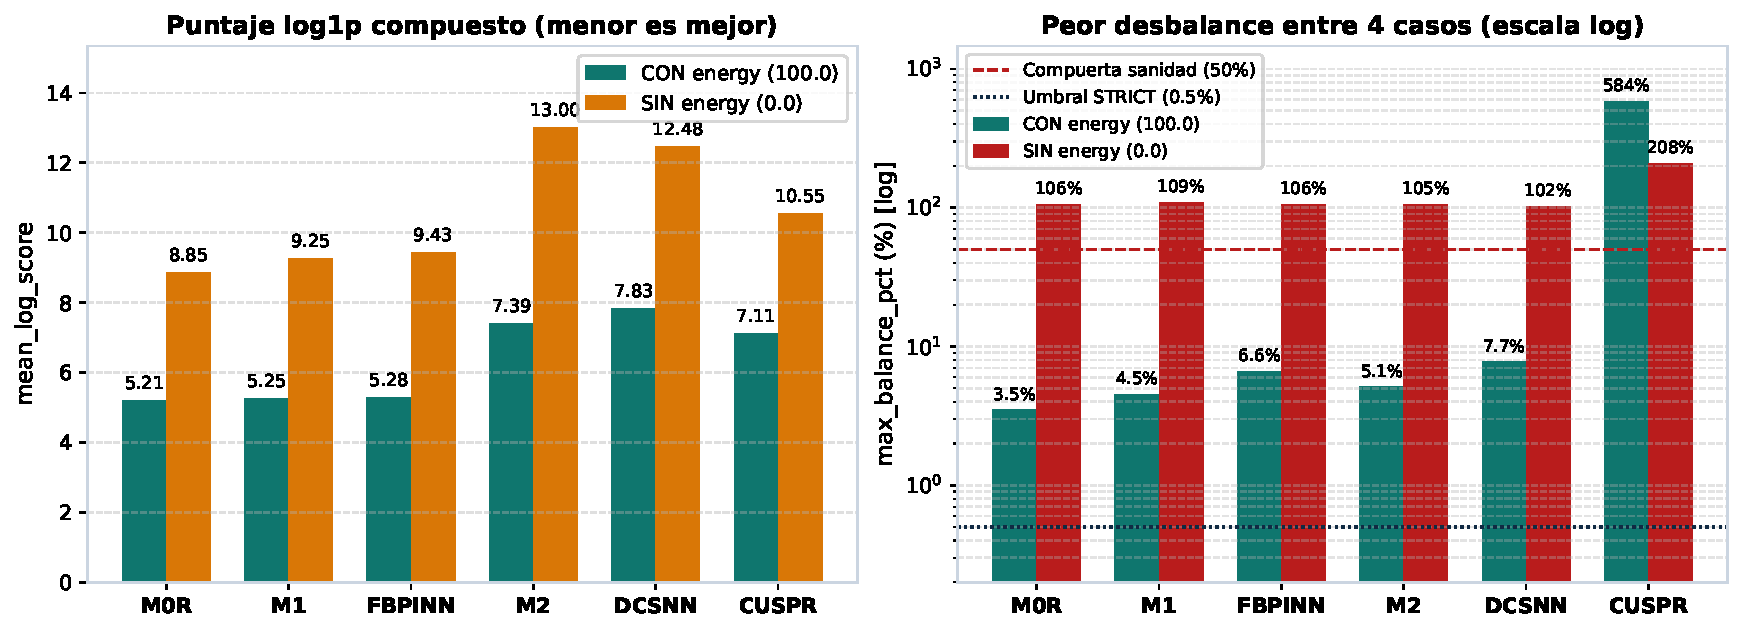
\includegraphics[width=0.95\textwidth,height=0.51\textheight,keepaspectratio]{figuras/fig_stage2_energy_impact.pdf}
  \vspace{0.08cm}
  \begin{cardbox}[Navy]{Conclusión física de la pasada dual}
    \small El término \texttt{energy = 100.0} es \textbf{indispensable} en cables multicapa: \textbf{todos} los clasificados ganaron con \texttt{CON energy} (bajando el desbalance de $>105\%$ a $<7.8\%$). La compuerta $\max(\text{bal}) < 50\%$ evita que modelos que solo pasan \texttt{STRICT} en \texttt{mms\_sine} ganen tras colapsar en cables.
  \end{cardbox}
\end{frame}

% SLIDE 25: ETAPA 2 RANKING FINAL
\begin{frame}{Etapa 2: Ranking Final, Promovidos y Descartados}
  \framesubtitle{Resultados oficiales en \hdrlink{../notebooks_campaign/campaign_workspace/promoted_models.json}{promoted\_models.json} (criterio \texttt{log1p} + compuerta $\text{bal} < 50\%$)}
  \centering
  \resizebox{0.99\textwidth}{!}{%
  \begin{tabular}{@{}clrrrrcl@{}}
    \toprule
    \textbf{\#} & \textbf{Modelo} & \textbf{Modo ganador} & \textbf{\texttt{log\_score}} & \textbf{NRMSE} & \textbf{$|\Delta T_{\max}|$} & \textbf{Max Bal.} & \textbf{Estado en embudo} \\
    \midrule
    \rowcolor{TealLight} 1 & \textbf{\texttt{M0R}} & CON energy (100) & \textbf{5.206} & 0.991\% & 1.297 K & \textbf{3.49\%} & \textbf{Promovido + Finalista 4B} \\
    \rowcolor{TealLight} 2 & \textbf{\texttt{M1}} & CON energy (100) & \textbf{5.253} & 0.840\% & \textbf{0.747 K} & \textbf{4.49\%} & \textbf{Promovido + Finalista 4B} \\
    3 & \textbf{\texttt{FBPINN}} & CON energy (100) & 5.279 & \textbf{0.639\%} & 0.888 K & 6.57\% & \textbf{Promovido a Etapa 3/4A} \\
    \rowcolor{RowAlt} 4 & \textbf{\texttt{M2}} & CON energy (100) & 7.389 & 5.324\% & 8.250 K & 5.11\% & \textbf{Promovido a Etapa 3/4A} \\
    5 & \textbf{\texttt{DCSNN}} & CON energy (100) & 7.827 & 5.354\% & 8.748 K & 7.75\% & \textbf{Promovido a Etapa 3/4A} \\
    \rowcolor{RowAlt} 6 & \texttt{M1\_EXACT} & CON energy (100) & 10.565 & 12.134\% & 36.584 K & 47.88\% & No promovido (Top 5 lleno) \\
    \midrule
    -- & \texttt{CUSPR} & CON energy (100) & 7.110 & 0.788\% & 1.097 K & \textcolor{Coral}{\textbf{584.23\%}} & Rechazado (\texttt{cable\_disk} bal) \\
    \rowcolor{CoralLight!50} -- & \texttt{CUSP\_EXACT} & SIN energy (0) & 12.151 & 11.856\% & 41.525 K & \textcolor{Coral}{2161.49\%} & Rechazado (\texttt{aras}, \texttt{disk}) \\
    -- & \texttt{M0} & CON energy (100) & 12.190 & 12.216\% & 40.465 K & \textcolor{Coral}{84.47\%} & Rechazado (\texttt{aras}, \texttt{xlpe}) \\
    \rowcolor{CoralLight!50} -- & \texttt{CUSP} & CON energy (100) & 13.089 & 11.818\% & 40.772 K & \textcolor{Coral}{2259.88\%} & Rechazado (\texttt{xlpe}, \texttt{aras}) \\
    \bottomrule
  \end{tabular}}
  \vspace{0.12cm}
  \begin{flushleft}
    {\small \textbf{Destacado}: \texttt{M0R}, \texttt{M1} y \texttt{FBPINN} forman el pelotón líder ($<1\%$ NRMSE promedio y $<6.6\%$ balance máximo).}
  \end{flushleft}
\end{frame}

% SLIDE 26: ETAPA 2 DESEMPEÑO POR CASO PIVOTE
\begin{frame}{Etapa 2: Desempeño de los 5 Promovidos por Caso Pivote}
  \framesubtitle{Consistencia entre dominio analítico (\texttt{mms\_sine}), disco, XLPE 5 regiones y ARAS plano 13 regiones}
  \centering
  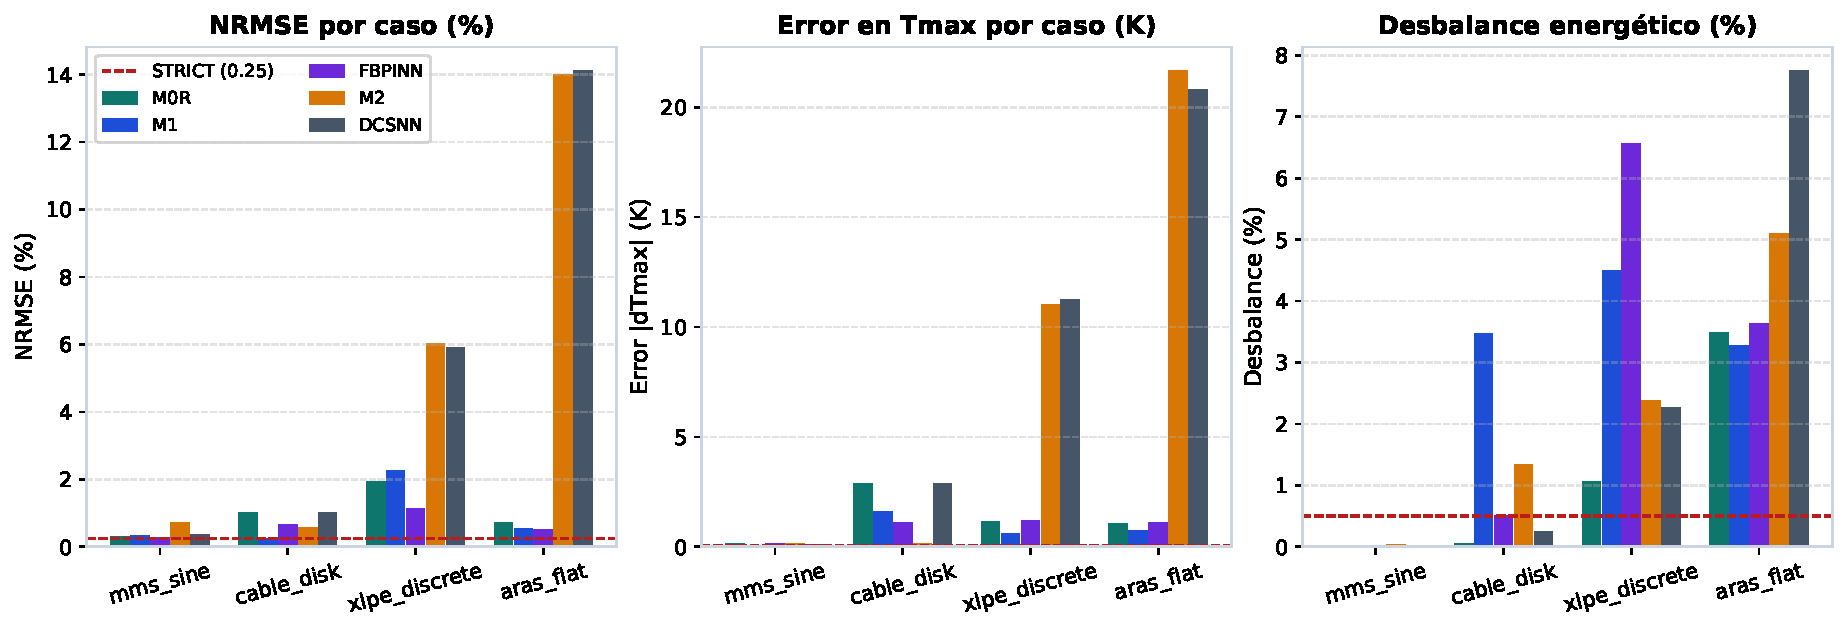
\includegraphics[width=0.97\textwidth,height=0.50\textheight,keepaspectratio]{figuras/fig_stage2_promoted_cases.pdf}
  \vspace{0.08cm}
  \begin{columns}[T,totalwidth=\textwidth]
    \begin{column}{0.49\textwidth}
      \begin{cardbox}[Teal]{Líderes en geometrías complejas}
        \small \texttt{M0R}, \texttt{M1} y \texttt{FBPINN} mantienen $\text{NRMSE} \le 0.72\%$ en \texttt{aras\_flat} y $\le 2.25\%$ en \texttt{xlpe\_discrete\_layers}.
      \end{cardbox}
    \end{column}
    \begin{column}{0.49\textwidth}
      \begin{cardbox}[Amber]{Brecha frente a \texttt{M2} y \texttt{DCSNN}}
        \small \texttt{M2} y \texttt{DCSNN} conservan energía en cables ($\text{bal} < 8\%$) pero alcanzan errores de $\sim 14\%$ en el plano trifásico \texttt{aras\_flat}.
      \end{cardbox}
    \end{column}
  \end{columns}
\end{frame}

% SLIDE 27: ETAPA 3 EN CURSO Y HOJA DE RUTA
\begin{frame}{Etapa 3 (Avance Actual) y Próximos Hitos (Etapas 4 y 5)}
  \framesubtitle{Instantánea real de \hdrlink{../notebooks_campaign/campaign_workspace/stage3_multicase_smoke/summary.json}{stage3\_multicase\_smoke/summary.json} mientras corre la campaña}
  \centering
  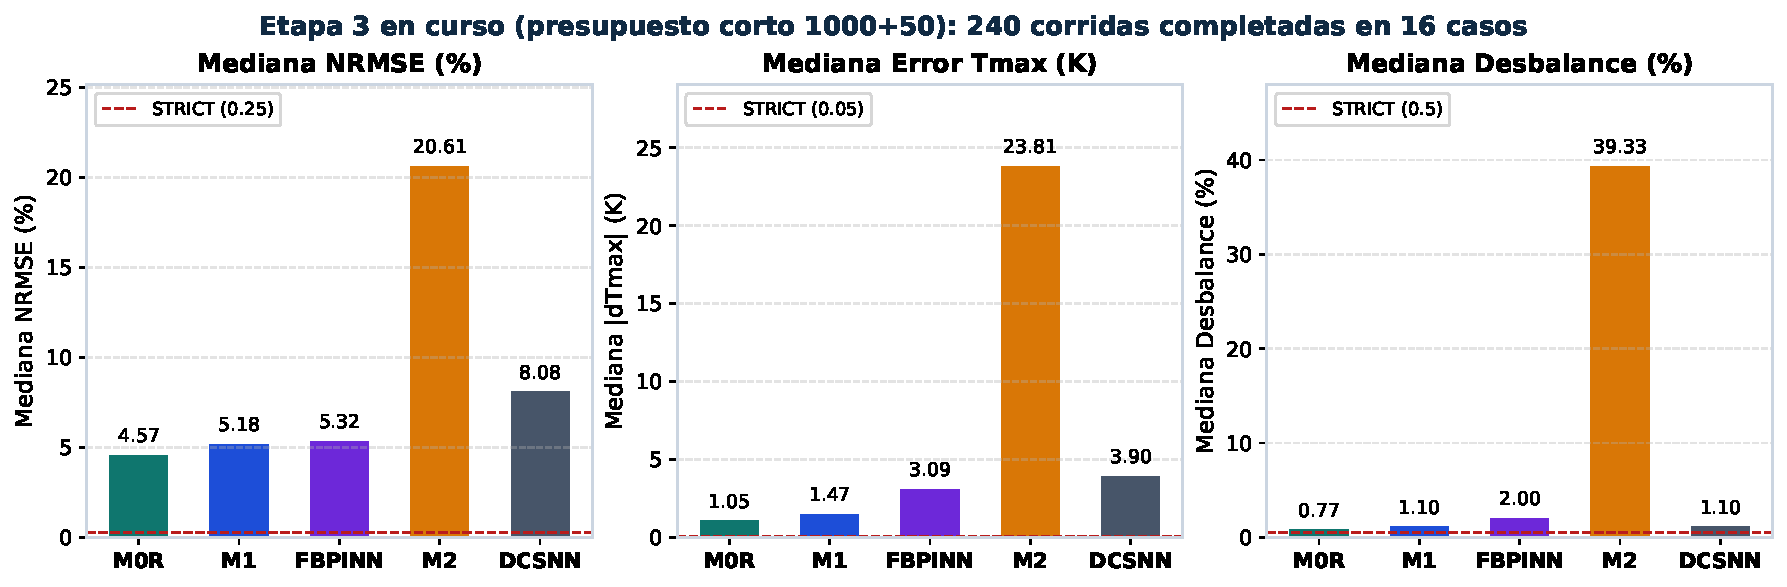
\includegraphics[width=0.95\textwidth,height=0.42\textheight,keepaspectratio]{figuras/fig_stage3_preliminar.pdf}
  \vspace{0.08cm}
  \begin{columns}[T,totalwidth=\textwidth]
    \begin{column}{0.49\textwidth}
      \begin{cardbox}[Teal]{Observación preliminar Etapa 3}
        \small \texttt{M0R} encabeza en mediana ($\text{NRMSE}=4.57\%$, $|\Delta T|=1.05\text{ K}$, $\text{bal}=0.77\%$), seguido muy de cerca por \texttt{M1} ($5.18\%$) y \texttt{FBPINN} ($5.32\%$).
      \end{cardbox}
    \end{column}
    \begin{column}{0.49\textwidth}
      \begin{cardbox}[Navy]{Próximos pasos tras completar Etapa 3}
        \small
        \begin{citemize}
          \item \textbf{\codelink{../notebooks_campaign/04_campana_adaptativa_y_corridas_largas.ipynb}{Etapa 4A/4B}}: convergencia profunda (\texttt{8000+20}) en \texttt{M0R} y \texttt{M1}.
          \item \textbf{\codelink{../notebooks_campaign/05_clasificacion_resultados_y_reporte_tesis.ipynb}{Etapa 5}}: tabla final \texttt{STRICT} y publicación Streamlit.
        \end{citemize}
      \end{cardbox}
    \end{column}
  \end{columns}
\end{frame}

% SLIDE 28: CIERRE Y LINKS DIRECTOS
\begin{frame}{Resumen Ejecutivo y Mapa de Navegación del Repositorio}
  \framesubtitle{Todos los módulos, documentación, casos, resultados y Front-End enlazados desde esta presentación}
  \begin{columns}[T,totalwidth=\textwidth]
    \begin{column}{0.49\textwidth}
      \begin{cardbox}[Navy]{Código fuente y modelos}
        \small
        \begin{citemize}
          \item Núcleo físico: \codelink{../src/pinn_thermal/core/problem.py}{problem.py}, \codelink{../src/pinn_thermal/core/objective.py}{objective.py}, \codelink{../src/pinn_thermal/core/trainer.py}{trainer.py}
          \item Artefactos y FEM: \codelink{../src/pinn_thermal/core/artifact.py}{artifact.py}, \codelink{../src/pinn_thermal/fem/runner.py}{fem/runner.py}
          \item Modelos: \codelink{../src/pinn_thermal/models/baseline.py}{baseline.py}, \codelink{../src/pinn_thermal/models/cusp.py}{cusp.py}, \codelink{../src/pinn_thermal/models/dcsnn.py}{dcsnn.py}, \codelink{../src/pinn_thermal/models/fbpinn.py}{fbpinn.py}, \codelink{../src/pinn_thermal/models/exact.py}{exact.py}
        \end{citemize}
      \end{cardbox}
    \end{column}
    \begin{column}{0.49\textwidth}
      \begin{cardbox}[Teal]{Campañas, Front-End y Documentación}
        \small
        \begin{citemize}
          \item Cuadernos: \codelink{../notebooks_campaign/02_screening_seleccion_modelos_1200_50.ipynb}{02\_screening}, \codelink{../notebooks_campaign/03_smoke_multicaso_semillas.ipynb}{03\_smoke}, \codelink{../notebooks_campaign/04_campana_adaptativa_y_corridas_largas.ipynb}{04\_campana}, \codelink{../notebooks_campaign/05_clasificacion_resultados_y_reporte_tesis.ipynb}{05\_reporte}
          \item Front-End: \codelink{../frontend/app.py}{frontend/app.py} \textbar\ \href{run:launch_frontend.bat}{\textcolor{Amber}{\underline{\textbf{Arrancar}}}} \textbar\ \href{http://localhost:8501}{\textcolor{Teal}{\underline{\texttt{localhost:8501}}}}
          \item Manuales: \codelink{../docs/detalle_tecnico_implementaciones_pinn.md}{detalle\_tecnico\_pinn.md}, \codelink{../docs/formato_json.md}{formato\_json.md}
        \end{citemize}
      \end{cardbox}
    \end{column}
  \end{columns}
\end{frame}

\end{document}
